\documentclass[dvipdfmx]{jsarticle}


\usepackage{tcolorbox}
\usepackage{color}
\usepackage{listings, plistings}

%% ノート/latexメモ
%% http://pepper.is.sci.toho-u.ac.jp/pepper/index.php?%A5%CE%A1%BC%A5%C8%2Flatex%A5%E1%A5%E2

%% JavaScriptの設定
%% https://e8l.hatenablog.com/entry/2015/11/29/232800
\lstdefinelanguage{javascript}{
  morekeywords = [1]{ %keywords
    await, break, case, catch, class, const, continue, debugger, default, delete, 
    do, else, enum, export, extends, finally, for, function, function*, if, implements, import, in, 
    instanceof, interface, let, new, package, private, protected, public, return, static, super,
    switch, this, throw, try, typeof, var, void, while, with, yield, yield*
  },
  morekeywords = [2]{ %literal
    false, Infinity, NaN, null, true, undefined
  },
  morekeywords = [3] { %Classes
    Array, ArrayBuffer, Boolean, DataView, Date, Error, EvalError, Float32Array, Float64Array,
    Function, Generator, GeneratorFunction, Int16Array, Int32Array, Int8Array, InternalError,
    JSON, Map, Math, Number, Object, Promise, Proxy, RangeError, ReferenceError, Reflect,
    RegExp, Set, String, Symbol, SyntaxError, TypeError, URIError, Uint16Array, Uint32Array,
    Uint8Array, Uint8ClampedArray, WeakMap, WeakSet
  },
  morecomment = [l]{//},
  morecomment = [s]{/*}{*/},
  morestring = [b]{"},
  morestring = [b]{'},
  alsodigit = {-},
  sensitive = true
}

%% 修正時刻: Tue 2022/03/15 10:04:41


% Java
\lstset{% 
  frame=single,
  backgroundcolor={\color[gray]{.9}},
  stringstyle={\ttfamily \color[rgb]{0,0,1}},
  commentstyle={\itshape \color[cmyk]{1,0,1,0}},
  identifierstyle={\ttfamily}, 
  keywordstyle={\ttfamily \color[cmyk]{0,1,0,0}},
  basicstyle={\ttfamily},
  breaklines=true,
  xleftmargin=0zw,
  xrightmargin=0zw,
  framerule=.2pt,
  columns=[l]{fullflexible},
  numbers=left,
  stepnumber=1,
  numberstyle={\scriptsize},
  numbersep=1em,
  language={Java},
  lineskip=-0.5zw,
  morecomment={[s][{\color[cmyk]{1,0,0,0}}]{/**}{*/}},
  keepspaces=true,         % 空白の連続をそのままで
  showstringspaces=false,  % 空白字をOFF
}
%\usepackage[dvipdfmx]{graphicx}
\usepackage{url}
\usepackage[dvipdfmx]{hyperref}
\usepackage{amsmath, amssymb}
\usepackage{itembkbx}
\usepackage{eclbkbox}	% required for `\breakbox' (yatex added)
\usepackage{enumerate}
\usepackage[default]{cantarell}
\usepackage[T1]{fontenc}
\fboxrule=0.5pt
\parindent=1em
\definecolor{mygrey}{rgb}{0.97, 0.97, 0.97}

\makeatletter
\def\verbatim@font{\normalfont
\let\do\do@noligs
\verbatim@nolig@list}
\makeatother

\begin{document}

%\anaumeと入力すると穴埋め解答欄が作れるようにしてる。\anaumesmallで小さめの穴埋めになる。
\newcounter{mycounter} % カウンターを作る
\setcounter{mycounter}{0} % カウンターを初期化
\newcommand{\anaume}[1][]{\refstepcounter{mycounter}{#1}{\boxed{\phantom{aa}\textnormal{\themycounter}\phantom{aa}}}} %穴埋め問題の空欄作ってる。
\newcommand{\anaumesmall}[1][]{\refstepcounter{mycounter}{#1}{\boxed{\tiny{\phantom{a}\themycounter \phantom{a}}}}}%小さい版作ってる。色々改造できる。

%% 修正時刻: Tue 2022/03/15 10:04:411


\section{テーブル(表)を作成する}

\subsection{作成する表のイメージ}

以下のような表を作成することとする。

\begin{table}[h]
 \caption{emp}
 \begin{center}
  \begin{tabular}[h]{|c|l|c|c|c|}
   \hline
   ID & 名前       & 年齢 & 誕生年 & 部署ID \\ \hline\hline
   1  & 菅原文太   & 40   & 1933   & 001    \\ \hline
   2  & 千葉真一   & 34   & 1939   & 002    \\ \hline
   3  & 北大路欣也 & 30   & 1943   & 003    \\ \hline
   4  & 梶芽衣子   & 26   & 1947   & 002    \\ \hline
  \end{tabular}
 \end{center}
\end{table}

\begin{table}[h]
 \caption{dept}
 \begin{center}
  \begin{tabular}{|l|c|} \hline
   ID   & 部署名 \\ \hline\hline
   001  & 総務部 \\ \hline
   002  & 営業部 \\ \hline
   003  & 経理部 \\ \hline
   004  & 開発部 \\ \hline
  \end{tabular}
 \end{center}
\end{table}

そして、上の2つの表から、以下の結合表を表示することとする。

\begin{table}[h]
 \begin{center}
  \begin{tabular}[h]{|c|l|c|c|c|}
   \hline
   ID & 名前       & 年齢  & 部署名 \\ \hline\hline
   1  & 菅原文太   & 40    & 総務部    \\ \hline
   2  & 千葉真一   & 34    & 営業部    \\ \hline
   3  & 北大路欣也 & 30    & 経理部    \\ \hline
   4  & 梶芽衣子   & 26    & 営業部    \\ \hline
  \end{tabular}
 \end{center}
\end{table}
 
\newpage
 
\subsection{テーブルの定義}

テーブルの定義を決める。

\begin{table}[ht]
 \caption{empテーブルの定義}
 \begin{center}
  \begin{tabular}{|l|l|l|} \hline
   項目 & 型 & オプション \\ \hline
   id   & int & primary key, auto\_increment \\ 
   name & varchar(20) & not null \\ 
   age  & int & not null \\ 
   birthday & year & not null \\ 
   dept\_id & char(3) & \\ \hline
  \end{tabular}
 \end{center}
\end{table}

\textgt{型}

\begin{tabular}{ll}
 int型 & 整数。これがよく使われる。 \\
 varchar型 & 可変長の文字列型。ここでは最大20文字としている。(全角文字を使った場合) \\
 year型 & 年のみを扱う型。誕生の年だけを入力する。 \\
 char型 & 固定長の文字型。ここでは半角で3文字としている。
\end{tabular}

\vspace{3mm}
\textgt{オプション}

\begin{tabular}{ll}
 primary key & 項目 id をデータの識別に使う。重複する値がないことが保証される。 \\
 auto\_increment & 自動連番。自動的に順に番号を振ってくれる機能を使う。 \\
 not null & 入力が必須。もしも入力しなかったら エラー になる。 \\
\end{tabular}

\vspace{3mm}
最後の dept\_id を not null にしなかったのは、部署ID のない社員もいるかもしれないからである。

\vspace{3mm}
deptテーブルは、このような定義になる。
 
\begin{table}[h]
 \caption{deptテーブルの定義}
 \begin{center}
  \begin{tabular}{|l|l|l|} \hline
   項目 & 型 & オプション \\ \hline
   id   & char(3) & primary key \\ 
   name & varchar(20) & not null \\ \hline
  \end{tabular}
 \end{center}
\end{table}

今回の場合、empテーブルには dept\_id が入っている。これは、deptテーブルの id のことである。
このことにより、empテーブルとdeptテーブルを結合させることができる。

このときの empテーブルの dept\_id のことを ``\textgt{外部キー}'' という。


\subsection{テーブルの作成}

テーブルを作成する前に、データベースの使用を宣言する。

\begin{tcolorbox}
 mysql$>$ USE \ sample; \hspace{20mm} \fbox{use \ データベース名 \,;}
\end{tcolorbox}

以下のコマンドにより empテーブルを作成できる。

\begin{lstlisting}[numbers=none]
 mysql> CREATE TABLE emp (
     ->   id INT AUTO_INCREMENT,
     ->   name VARCHAR(20) NOT NULL,
     ->   age INT NOT NULL,
     ->   birthday YEAR NOT NULL,
     ->   dept_id CHAR(3),
     ->   PRIMARY KEY (id)
     -> );
\end{lstlisting}

同様に deptテーブルも作成する。
\footnote{primary key の指定は、id の指定のときに書くこともできるし、別項目に分けて書くこともできる。}

\begin{lstlisting}[numbers=none]
 mysql> CREATE TABLE dept (
     ->   id CHAR(3) PRIMARY KEY,
     ->   name VARCHAR(20) NOT NULL
     -> );
\end{lstlisting}

\vspace{3mm}
\noindent ※
\quad 作成したテーブルの構造は以下のコマンドで確認できる。 \\
mysql$>$ \textsf{desc emp;}
\begin{verbatim}
+----------+-------------+------+-----+---------+----------------+
| Field    | Type        | Null | Key | Default | Extra          |
+----------+-------------+------+-----+---------+----------------+
| id       | int(11)     | NO   | PRI | NULL    | auto_increment |
| name     | varchar(20) | NO   |     | NULL    |                |
| age      | int(11)     | NO   |     | NULL    |                |
| birthday | year(4)     | NO   |     | NULL    |                |
| dept_id  | char(3)     | YES  |     | NULL    |                |
+----------+-------------+------+-----+---------+----------------+
\end{verbatim}

また、テーブルを作成したときのコマンドは以下で確認できる。\\
mysql$>$ \textsf{show create table emp;}
\begin{verbatim}
...(省略)... 
CREATE TABLE `emp` ( 
  `id` int(11) NOT NULL AUTO_INCREMENT,
  `name` varchar(20) NOT NULL,
  `age` int(11) NOT NULL,
  `birthday` year(4) NOT NULL,
  `dept_id` char(3) DEFAULT NULL,
  PRIMARY KEY (`id`)
) ENGINE=InnoDB DEFAULT CHARSET=utf8mb4
\end{verbatim}

\subsection{データの登録}

データの登録は、以下のコマンドでできる。

\begin{lstlisting}[numbers=none, language=sql]
 mysql> INSERT INTO emp (name, age, birthday, dept_id) VALUES ('菅原文太', 40, 1933, '001');
\end{lstlisting}

\begin{tabular}{|l|} \hline
 INSERT \ INTO \ テーブル名
 ( \ カラム名1, \ カラム名2, \ カラム名3, \ \dots \dots \ ) \ VALUES \ (データ1, \\
 データ2, \ データ3, \ \dots \dots) \\ \hline
\end{tabular}


\rightline{※ 各データの区切りは \textsf{,}(カンマ)}
\noindent
''id'' は auto\_increment(自動連番) なので、指定しない。\\
また、dept\_id は char(3) なので、\textsf{'001'} シングルクォーテーションを使って入力する。

画面の関係で一行で入力しづらければ、次のように二行で入力することもできる。

\begin{lstlisting}[numbers=none, language=sql]
 mysql> INSERT INTO emp (name, age, birthday, dept_id)
     -> VALUES ('千葉真一', 34, 1939, '002');
\end{lstlisting}

TeraPad などのエディタで記述しておいて、コピー\&貼り付け ですることもできる。

以下のようにすると、一度で入力できてしまう。

\begin{lstlisting}[numbers=none, language=sql]
 mysql> INSERT INTO emp (name, age, birthday, dept_id) VALUES
     -> ('北大路欣也', 30, 1943, '003'),
     -> ('梶芽衣子', 26, 1947, '002');
\end{lstlisting}

これも、エディタに記述しておいて、コピー\&貼り付けでも できる。

データの確認は次のコマンドでできる。

\begin{tcolorbox}
 mysql$>$ \textsf{SELECT * FROM emp;}
\end{tcolorbox}

\rightline{\fbox{SELECT \ * \ FROM \ テーブル名}}

\begin{verbatim}
+----+------------+-----+----------+---------+
| id | name       | age | birthday | dept_id |
+----+------------+-----+----------+---------+
|  1 | 菅原文太   |  40 |     1933 | 001     |
|  2 | 千葉真一   |  34 |     1939 | 002     |
|  3 | 北大路欣也 |  30 |     1943 | 003     |
|  4 | 梶芽衣子   |  26 |     1947 | 002     |
+----+------------+-----+----------+---------+
\end{verbatim}

同様に、deptテーブルについてもデータを登録する。

\begin{lstlisting}[numbers=none, language=sql]
mysql> INSERT INTO dept (id, name) VALUES
    -> ('001', '総務部'),
    -> ('002', '営業部'),
    -> ('003', '経理部'),
    -> ('004', '開発部');
\end{lstlisting}

確認する。

\begin{lstlisting}[numbers=none, language=sql]
 mysql> SELECT * FROM dept;
\end{lstlisting}

\begin{verbatim}
+-----+--------+
| id  | name   |
+-----+--------+
| 001 | 総務部 |
| 002 | 営業部 |
| 003 | 経理部 |
| 004 | 開発部 |
+-----+--------+
\end{verbatim}

\section{練習問題}

\subsection{テーブル作成問題(1)}

以下のようなテーブル person を作成してください。

\vspace{3mm}
\begin{tabular}{|c|l|c|c|c|l|} \hline
 ID & 名前        & 性別  & 誕生日     & 出身      & コース            \\ \hline\hline
  1 & 染谷将太    & 男    & 1992-09-03 & 東京都    & JavaScriptコース  \\ \hline 
  2 & 二階堂ふみ  & 女    & 1994-09-21 & 沖縄県    & PHPコース         \\ \hline 
  3 & 渡辺哲      & 男    & 1950-03-11 & 愛知県    & Javaコース        \\ \hline 
  4 & 窪塚洋介    & 男    & 1979-05-07 & 神奈川県  & HTML/CSSコース    \\ \hline 
  5 & 吉高由里子  & 女    & 1988-07-22 & 東京都    & Javaコース        \\ \hline
\end{tabular}
\vspace{3mm}

データ型
\vspace{-3mm}
\begin{itemize}
 \item ID --- id, INT型、自動連番、主キー
 \item 名前 --- name, VARCHAR型、(20)くらいにしておく。(全角でも半角でも)。
 \item 性別 --- gender, CHAR型、(1)なら1文字(全角でも半角でも)
 \item 誕生日 --- birthday, DATE型。
 \item 出身 --- state, VARCHAR型、(5) で全ておさまる。(10)でもよい。
 \item コース --- course, VARCHAR型、(50)くらいにする。
\end{itemize}

\newpage
\subsection{テーブル作成問題(2)}

このテーブルは、以下のように 4つ のテーブルに分けて管理しようと思います。

\begin{multicols}{2}
\vspace{3mm}
gender表 \\
\begin{tabular}{|c|c|} \hline
 \underline{ID}  & 識別名 \\ \hline\hline
 0   & 不明 \\ \hline
 1   & 男性  \\ \hline
 2   & 女性  \\ \hline
 3   & その他 \\ \hline
\end{tabular}
\vspace{3mm}

\columnbreak

gender表定義
\begin{itemize}
 \item ID --- gid, 主キー、CHAR(1)
 \item 識別名 -- gname, VARCHAR(3)
\end{itemize} 

\end{multicols}

 
\begin{multicols}{2}

\vspace{3mm}
state表 \\
\begin{tabular}{|c|l|} \hline
 \underline{ID} & 都道府県名 \\ \hline\hline
 01   & 北海道 \\ \hline
 02   & 青森県 \\ \hline
 03   & 岩手県 \\ \hline
 04   & 宮城県 \\ \hline
 \dots & \dots \\ \hline
 47   & 沖縄県  \\ \hline
\end{tabular}
\vspace{3mm}

\columnbreak

state表定義
\begin{itemize}
 \item ID --- sid, 主キー、CHAR(2)
 \item 都道府県 -- sname, VARCHAR(5)
\end{itemize} 

 state表の入力データは別途あります。(state.sql)
\end{multicols}


\begin{multicols}{2}

\vspace{3mm}
course表 \\
\begin{tabular}{|c|l|} \hline
 \underline{ID} & コース名 \\ \hline\hline
 1   & HTML/CSSコース \\ \hline
 2   & JavaScriptコース \\ \hline
 3   & PHPコース \\ \hline
 4   & Javaコース \\ \hline
 5   & サーブレットJSPコース  \\ \hline
\end{tabular}
\vspace{3mm}

\columnbreak
 
course表定義
\begin{itemize}
 \item ID --- cid, int型、主キー、自動連番
 \item コース名 -- cname, VARCHAR(50)
\end{itemize} 

 
\end{multicols}


 person表 は、以下のように変更する必要があります。

\begin{multicols}{2}
\vspace{3mm}
person表 \\
\begin{tabular}{|c|l|c|c|c|l|} \hline
 ID & 名前        & g\_id  & 誕生日     & s\_id  & c\_id  \\ \hline\hline
  1 & 染谷将太    &  1    & 1992-09-03 & 13    & 2     \\ \hline 
  2 & 二階堂ふみ  &  2    & 1994-09-21 & 47    & 3     \\ \hline 
  3 & 渡辺哲      &  1    & 1950-03-11 & 23    & 4     \\ \hline 
  4 & 窪塚洋介    &  1    & 1979-05-07 & 14    & 1     \\ \hline 
  5 & 吉高由里子  &  2    & 1988-07-22 & 13    & 4     \\ \hline
\end{tabular}
\vspace{3mm}
 
\columnbreak

person表定義
\begin{itemize}
 \item ID --- (そのまま)
 \item 名前 --- (そのまま)
 \item 性別 --- g\_id, CHAR(1)
 \item 誕生日 --- (そのまま)
 \item 出身 --- s\_id, CHAR(2)
 \item コース --- c\_id, INT型、
\end{itemize}

\end{multicols}



\newpage
\section{ファイル読込みによるデータの登録}

同様のことを、
登録のための SQL文を外部ファイルに記述しておいて、
それを読み込むという方法でもできる。
dept表を例にして説明する。

\subsubsection{作業のためのフォルダを用意して、そこでファイルをつくる。}

ファイルを置くためのフォルダを用意する。
ここでは仮に、ドキュメントフォルダに mysql というフォルダを作成したとする。

そこに、以下の内容のファイル ''insert\_dept.sql'' を作成する。

\begin{lstlisting}[caption=insert\_dept.sql, language=sql]
-- dept テーブル

INSERT INTO dept (id, name) VALUES
('001', '総務部'),
('002', '営業部'),
('003', '経理部'),
('004', '開発部');
\end{lstlisting}

{-}{-} で始まる行は、コメントである。
\footnote{ほかに、\# で始まる行もコメント。また複数行は、/* ... */ が使える。}

また、SQLのコマンドは大文字で記述したほうがよい。
コマンドプロンプトでは、小文字でかまわないが、このようにファイルとして記述する場合は、
SQLのコマンド文字列は大文字で記述し、ユーザーが用意した変数などは小文字で記述しておく。
あとで見なおしたりする場合にわかりやすい。


\subsubsection{そのフォルダでコマンドプロンプトを起動する。}

そのフォルダでコマンドプロンプトを起動する。
次の図のようにする。

\vspace{3mm}
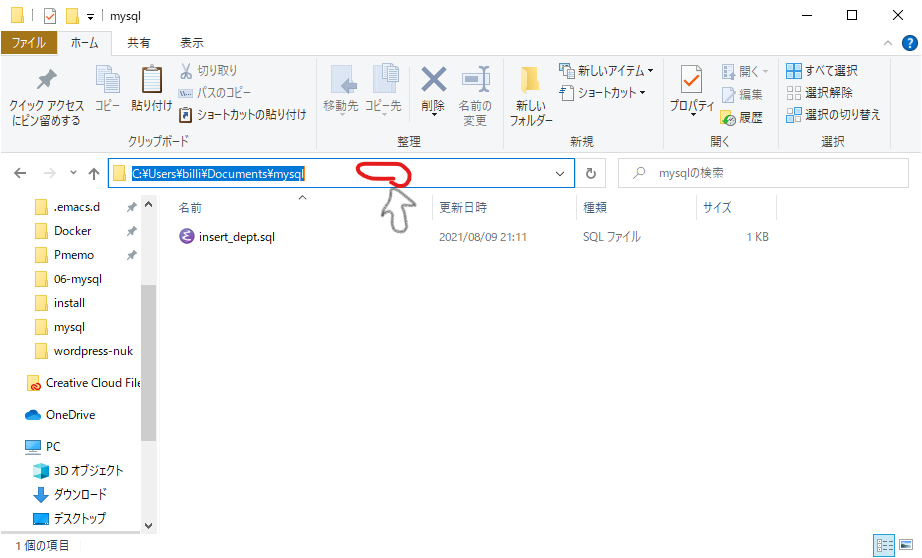
\includegraphics[width=10cm]{../06-mysql/03-cmd.png}
\vspace{3mm}

上の図のように、エクスプローラのアドレス欄の余白部分をクリックする。
すると、現在のフォルダをあらわす文字列が青く反転する。

\vspace{3mm}
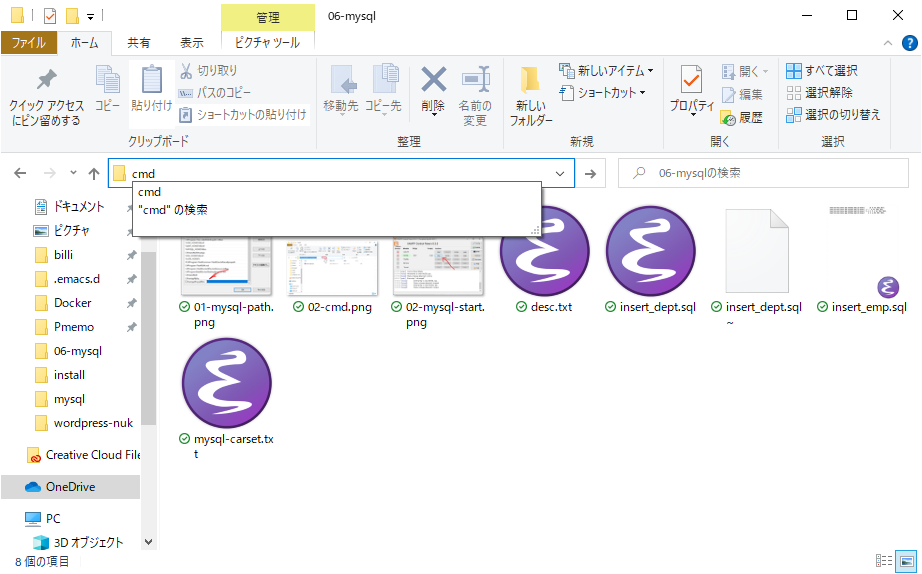
\includegraphics[width=10cm]{../06-mysql/04-cmd.png}
\vspace{3mm}

上の図のように、そこに ''\textsf{cmd}'' と入力して Enterキーを押下する。
すると、そのフォルダでコマンドプロンプトが起動する。

\vspace{3mm}
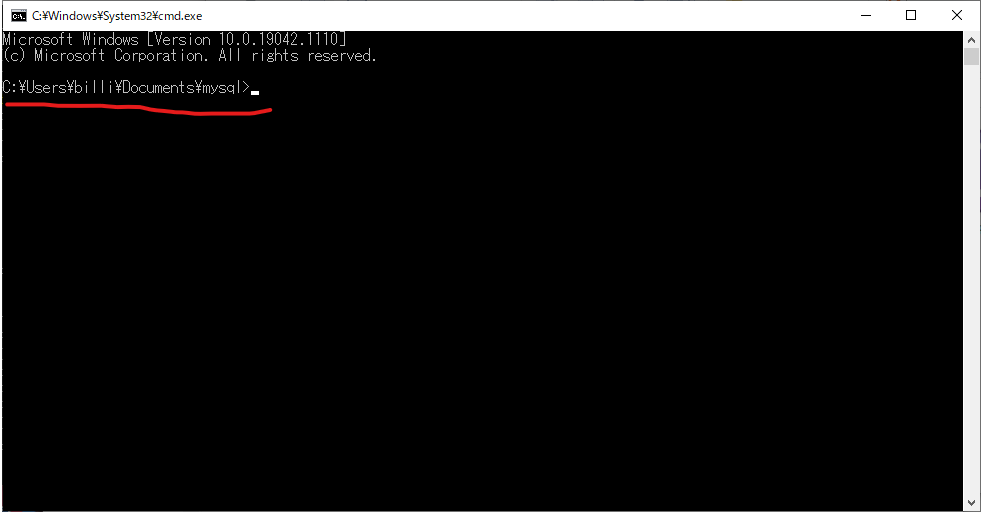
\includegraphics[width=11cm]{../06-mysql/05-cmd.png}
\vspace{3mm}

上の図の赤い線の部分が、現在のフォルダになっている。

\begin{tcolorbox}
 C:\yen Users\yen (ユーザー名)\yen Documents\yen mysql$>$ \textsf{dir}
\end{tcolorbox}

\textsf{dir} というコマンドを実行すると、現フォルダのファイルが一覧できる。
\textsf{insert\_dept.sql} があることがわかる。

\begin{verbatim}
 2021/08/09  22:05   <DIR>       .                    (このフォルダ)
 2021/08/09  22:05   <DIR>       ..                   (ひとつ上の階層)
 2021/08/09  22:05          222  insert_dept.sql  
\end{verbatim}


\subsubsection{ファイルを読み込んで、SQL文を実行する}

ここで、mysqlサーバーに接続する。

\begin{lstlisting}[numbers=none, language=sql]
C:\Users\(ユーザー名)\Documents\mysql> mysql -u sampleuser -p
 Password: ********
\end{lstlisting}

\textsf{sample}データベースの使用を宣言する。

\begin{lstlisting}[numbers=none, language=sql]
 mysql> USE sample;
\end{lstlisting}

先ほど作った dept表は削除する。

\begin{lstlisting}[numbers=none, language=sql]
 mysql> DROP TABLE dept;
\end{lstlisting}

次に、以下のコマンドで \textsf{insert\_dept.sql} を実行できる。

\begin{lstlisting}[numbers=none, language=sql]
 mysql> source insert_dept.sql
\end{lstlisting}

あるいは、以下のような省略形もある。

\begin{lstlisting}[numbers=none, language=sql]
 mysql> \. insert_dept.sql
\end{lstlisting}

確認する。

\begin{lstlisting}[numbers=none, language=sql]
 mysql> SELECT * FROM dept;
\end{lstlisting}

\begin{verbatim}
+-----+--------+
| id  | name   |
+-----+--------+
| 001 | 総務部 |
| 002 | 営業部 |
| 003 | 経理部 |
| 004 | 開発部 |
+-----+--------+
\end{verbatim}

読み込めているのがわかる。


\subsection{テーブル作成からデータの登録までを自動化する}

このことを応用して、テーブルの作成からデータの登録までを、ファイル読込みによって
自動化することができる。

以下のような記述が考えられる。

\begin{lstlisting}[
 caption=init\_data.sql,
 language=sql
]
 CREATE DATABASE sample;

 -- sample データベースを使用
 USE sample;
 
 -- emp テーブルの作成
 CREATE TABLE emp (
   id INT AUTO_INCREMENT,
   name VARCHAR(20) NOT NULL,
   age INT NOT NULL,
   birthday YEAR NOT NULL,
   dept_id CHAR(3),
   PRIMARY KEY (id)
 );

 -- dept テーブルの作成
 CREATE TABLE dept (
   id CHAR(3) PRIMARY KEY,
   name VARCHAR(20) NOT NULL
 );

 INSERT INTO emp (name, age, birthday, dept_id) VALUES
 ('菅原文太', 40, 1933, '001'),
 ('千葉真一', 34, 1939, '002') ,
 ('北大路欣也', 30, 1943, '003'),
 ('梶芽衣子', 26, 1947, '002');

 INSERT INTO dept (id, name) VALUES
 ('001', '総務部'),
 ('002', '営業部'),
 ('003', '経理部'),
 ('004', '開発部');

 SELECT * FROM emp;
 SELECT * FROM dept;
\end{lstlisting}

データベースを削除してから、これを実行する。

\begin{tcolorbox}
 mysql$>$ drop database sample; \\
 mysql$>$ \yen . init\_data.sql
\end{tcolorbox}

データベースが再度作成されたのがわかる。

今回は、データベースを削除して、再度作り直したが、
データベースを削除せずに、初期状態に戻すには、
以下のようにする必要がある。

\begin{enumerate}
 \item データベースが存在しなかったら、データベースを作成する。
 \item テーブルが存在していたら、それを削除してから、テーブルを作成して、
       データを挿入する。
 \item 自動連番は、1から始まるようにしておく。
\end{enumerate}

テーブルを削除しているのは、もしそのテーブルが存在していたとしても、
その中のデータがすでに改変されてしまっているかもしれないので、
初期状態に戻すには、テーブルを削除する必要があるからである。

それらも含めてスクリプトを作成すると、以下のようになる。

\begin{lstlisting}[
 caption=init\_data.sql,
 language=sql
]
 -- もし存在していなかったら sample データベースを作成する
 CREATE DATABASE IF NOT EXISTS sample;

 -- sample データベースを使用
 USE sample;
 
 -- emp テーブルの作成
 -- もし empテーブルが存在していたら削除する。
 -- その empテーブルの定義がこれから作成するのと同じという保証がないからである。

 DROP TABLE IF EXISTS emp;
 
 CREATE TABLE emp (
   id INT AUTO_INCREMENT,
   name VARCHAR(20) NOT NULL,
   age INT NOT NULL,
   birthday YEAR NOT NULL,
   dept_id CHAR(3),
   PRIMARY KEY (id)
 );

 -- dept テーブルの作成
 -- もし deptテーブルが存在していたら削除する。
 DROP TABLE IF EXISTS dept; 
 
 CREATE TABLE dept (
   id CHAR(3) PRIMARY KEY,
   name VARCHAR(20) NOT NULL
 );

 -- 自動連番を初期化する。
 ALTER TABLE emp AUTO_INCREMENT = 1;
 
 INSERT INTO emp (name, age, birthday, dept_id) VALUES
 ('菅原文太', 40, 1933, '001'),
 ('千葉真一', 34, 1939, '002') ,
 ('北大路欣也', 30, 1943, '003'),
 ('梶芽衣子', 26, 1947, '002');

 INSERT INTO dept (id, name) VALUES
 ('001', '総務部'),
 ('002', '営業部'),
 ('003', '経理部'),
 ('004', '開発部');

 SELECT * FROM emp;
 SELECT * FROM dept;
\end{lstlisting}

これにより、いつでもデータを初期状態に戻すことができるようになった。


\end{document}

%% 修正時刻: Sat May  2 15:10:04 2020


%% 修正時刻: Sun Feb 20 16:40:35 2022
